\documentclass[]{beamer}
\usepackage[utf8x]{inputenc}
\usepackage{pgfpages}
\usepackage{hyperref}
\usepackage{listings}
\usepackage{lstautogobble}
\usepackage{xspace}
\usepackage{xparse}
\usepackage{matlab-prettifier}
%\setbeameroption{show notes on second screen}

\usepackage{microtype}

\usepackage{tikz}
\usetikzlibrary{shapes.callouts, shapes.geometric, arrows, arrows.meta, chains}

% speech bubbles
\tikzset{
  invisible/.style={opacity=0,text opacity=0},
  visible on/.style={alt=#1{}{invisible}},
  alt/.code args={<#1>#2#3}{%
    \alt<#1>{\pgfkeysalso{#2}}{\pgfkeysalso{#3}} % \pgfkeysalso doesn't change the path
  },
}
\newcommand{\tikzmark}[1]{\tikz[overlay,remember picture,baseline=-0.5ex] \node (#1) {};}

\NewDocumentCommand{\mycallout}{r<> O{opacity=0.8,text opacity=1} m m}{%
  \tikz[remember picture, overlay]\node[align=center, fill=blue!20, text width=15em,
  #2,visible on=<#1>, rounded corners,
  draw,rectangle callout,anchor=pointer,callout relative pointer={(230:3em)}]
  at (#3) {#4};
}

% flowcharts
\tikzset{
  reg/.style={
    rectangle,
    rounded corners,
    minimum width=3cm,
    minimum height=1cm,
    align=center,
    draw=black
  },
  arrow/.style={thick,->},
  fade/.style={
    rectangle,
    rounded corners,
    minimum width=3cm,
    minimum height=1cm,
    align=center,
    draw=gray!30,
    text=gray!30,
  },
  fadearrow/.style={thick,->, gray!30},
  highlight/.style={
    rectangle,
    rounded corners,
    minimum width=3cm,
    minimum height=1cm,
    align=center,
    draw=black,
    fill=blue!10
  },
  end/.style={
    tape,
    tape bend top=none,tape bend height=2mm,
    tape bend bottom=out and in,
    minimum width=3cm,
    minimum height=1cm,
    align=center,
    draw=black
  },
  fadeend/.style={
  tape,
  tape bend top=none,tape bend height=2mm,
  tape bend bottom=out and in,
  minimum width=3cm,
  minimum height=1cm,
  align=center,
  draw=gray!30,
  text=gray!30
  }
}

\lstset{ %
  language=Matlab,
  style=Matlab-editor,
  autogobble=true,
  escapechar=!
}

\newcommand{\pct}{\texttt{\symbol{37}}}
\newcommand{\dir}{\texttt{\symbol{62}}}
\newcommand{\res}{\texttt{\symbol{60}}}
\newcommand{\lcb}{\texttt{\symbol{123}}}
\newcommand{\rcb}{\texttt{\symbol{125}}}
\newcommand{\lsb}{\texttt{\symbol{91}}}
\newcommand{\rsb}{\texttt{\symbol{93}}}
\newcommand{\keyword}[1]{\textcolor{blue}{#1}}
\newcommand{\lr}{\textsc{LabMate}}
\newcommand{\repo}{\url{https://github.com/msp-strath/LabMate}}
\newcommand{\ma}{\textsc{Matlab}}
\newcommand{\List}{\mathsf{List}}
\newcommand{\Unit}{\mathsf{Unit}}
\newcommand{\Abel}{\mathsf{Abel}}
\newcommand{\Int}{\mathsf{Int}}
\newcommand{\Matrix}{\mathsf{Matrix}}
\newcommand{\Enum}{\mathsf{Enum}}
\newcommand{\LL}{\mathsf{L}}
\newcommand{\TT}{\mathsf{T}}
\newcommand{\MM}{\mathsf{M}}
\newcommand{\Kg}{\mathsf{kg}}
\newcommand{\Sec}{\mathsf{s}}
\newcommand{\Km}{\mathsf{m}}
\newcommand{\NameTimes}{\!\!\times\!\!}


%\usepackage[backend=biber, style=apa, citestyle=apa, isbn=false, doi=false]{biblatex}
%\bibliography{labrat}

\setbeamertemplate{frametitle}[default][center]
\title{\huge \lr: \\ \centerline{an interactive assistant for \ma} }
\author[McBride, Nakov, Nordvall Forsberg]{\small Conor McBride, \underline{Georgi Nakov}, Fredrik Nordvall Forsberg}
\institute[]{University of Strathclyde}

\begin{document}

\begin{frame}
  \titlepage
\end{frame}

\begin{frame}[fragile]{Motivation}
\begin{itemize}[<+->]
\item A lot of metrology and testing software involves complex processing of data in various formats, converting between multiple units of measure
\item And lot of that software is implemented in \ma
\item A good and common practice is to document the \keyword{structure} and \keyword{significance} of each variable
\begin{lstlisting}[basicstyle=\small]
  function x_d = trajectory(x, ...)
  % x is the vector of angular positions
  % of the actuators, a 4x1 double
  R = 6371e3; % Earth radius in metres
  laa = vehicle(1)*pi/180; % Lat of vehicle in radians
  ...
\end{lstlisting}
\end{itemize}
\end{frame}

\begin{frame}{Motivation}
  These comments are a treasure trove:
  \begin{itemize}[<+->]
    \item convey \keyword{information vital for comprehension} of that software
    \item written by the user for other human users, and expressing \keyword{intent}
    \begin{itemize}
      \item and completely invisible to the machine
    \end{itemize}
    \item although in free form, the prose is \keyword{semi-structured} with emerging patterns
  \end{itemize}
  \visible<5->{\lr{} is our attempt to unearth the hidden riches.}
\end{frame}

\begin{frame}[fragile]{Living with(in) \ma}
\lr{} --- a processor and a language of \keyword{formal \ma{} comments}
\pause
\begin{itemize}[<+->]
  \item enhances the experience of working with the existing toolchains
  \begin{itemize}
    \item rather than insisting on adopting a totally new language
  \end{itemize}
  \item requests (input) to \lr\,, i.e., \keyword{directives}:\\
  \begin{center}
  \begin{tabular}{p{8em}p{4em}l}
    &  & $\pct\lcb$ \\
    $\pct\dir\;\mathit{directive}$& or & $\quad\dir\;\mathit{multiline\;directive}$  \\
    &  & $\pct\rcb$ \\
  \end{tabular}
  \end{center}
  \item responses (output) from \lr:
  \begin{center}
  \begin{tabular}{p{8em}p{4em}p{9.3em}}
    &  & $\pct\res\lcb$ \\
    $\pct\res\;\mathit{response}$& or & $\mathit{synthesized}\; \ma\;\mathit{code}$  \\
    &  & $\pct\res\rcb$ \\
  \end{tabular}
  \end{center}
    \item can be integrated into editors as an optional processing step
  \item run iteratively to maintain a dialogue with the user
\end{itemize}
\end{frame}

\begin{frame}{Classifying directives}
  What can \lr\ do for us?\pause
\begin{itemize}[<+->]
  \item perform \keyword{systematic transformation} of the user's code, e.g., consistently renaming all occurrences of a given variable;
  \item \keyword{generate} low-level \keyword{code} serving some stated high-level purpose via supplied metadata, e.g., to read a data set from a file.
  \item offer means to document \keyword{types} of functions and variables
  \begin{itemize}
    \item provide richer metadata, e.g., units of measure;
  \end{itemize}
  \item \keyword{query} the type of a part of the program
\end{itemize}
\end{frame}

\begin{frame}[fragile]{Code transformations}
Renaming a variable is perhaps the simplest and most common refactoring action\pause
 \begin{itemize}[<+->]
   \item \lstinline|%> rename x y|
   \item happens \keyword{simultaneously} and \keyword{transactionally} with all the other rename directives
   \begin{itemize}
     \item if all renamings \keyword{succeed}, notify the user: \lstinline|%< renamed x y|
     \item if any renaming \keyword{fails}, do not change the file...
   \end{itemize}
   \item but how can renaming fail?
 \end{itemize}
\end{frame}


\begin{frame}{Insights into scope management}
When exactly should renaming fail? \pause
\begin{itemize}
  \item renaming should be \keyword{non-capturing}, i.e., keep distinct variables distinct
\end{itemize}
\pause
\begin{columns}
  \begin{column}{0.4\textwidth}
    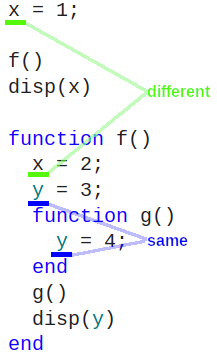
\includegraphics[width=0.3\paperwidth, keepaspectratio]{renaming.png}
  \end{column}
  \begin{column}{0.5\textwidth}
  \keyword{Scope of a variable}:
  \begin{itemize}[<+->]
    \item a variable defined at the \keyword{top level of the script} is distinct from a variable defined in a function (even if they share the same name)
    \item a variable defined \keyword{in a function} $f$ is visible to any nested functions of $f$
  \end{itemize}
  \visible<5->{\keyword{Observation}: two subsequent renamings $x \mapsto y \mapsto x$ must not change the meaning of the program}
  \vspace{3em}
  \end{column}
\end{columns}
\end{frame}


\begin{frame}{Code generation}
There are lot of menial programming tasks in the wild\pause
\begin{itemize}[<+->]
  \item e.g., code that handles data serialisation
  \begin{itemize}
    \item have to keep in mind what input is required, what are the dimensions, what format, etc...
    \item but this is metainformation, not necessarily evident in the \ma{} implementation
  \end{itemize}
\end{itemize}
\visible<5->{We can do better}
\pause
\begin{itemize}[<+->]
  \item develop a high-level \keyword{metalanguage of descriptions}
  \item read and validate descriptions, make sanity checks and generate \ma{} code that closely resembles hand crafted one
\end{itemize}
\end{frame}

\begin{frame}[fragile]{Code generation}
 \begin{columns}
   \begin{column}{0.45\textwidth}
    \begin{lstlisting}[basicstyle=\small]
%{
  > input readFromDisk
  myStruct :
    count : @Int
    totalLen : @Km
    unitLens : @count elements of @m
%}
    \end{lstlisting}
   \end{column}
   \begin{column}{0.45\textwidth}
   \begin{lstlisting}[basicstyle=\tiny]
%<{
  function myStruct = readFromDisk(fname);
  f1 = fopen(fname);
  c1 = textscan(f1, `%f`);
  src = c1{1};
  fclose(f1);
  readPtr = 1;
  myStruct.count = src[readPtr];
  readPtr = readPtr + 1;
  myStruct.totalLen = src[readPtr];
  readPtr = readPtr + 1;
  for i = 1:myStruct.count
    myStruct.unitLens[i] = src[readPtr + i];
  end
%>}
   \end{lstlisting}
   \end{column}
 \end{columns}
\end{frame}

\begin{frame}[fragile]{Types as machine-checkable documentation}
Types are a well established method of \keyword{communication} between the user and the machine.\pause\\
\vspace{1em}
\lr{} should enable the user to: \pause
\begin{itemize}[<+->]
  \item \keyword{annotate} variables with type information\\
  \begin{center}
    \lstinline|%> n :: int|
  \end{center}
  \begin{itemize}
    \item support \keyword{inferring} the types of most variables, thus eliminating the need for thorough annotations
  \end{itemize}
  \item make sure a specific type \keyword{admits} some \ma{} expression
  \begin{center}
    \lstinline|%> typecheck int n|
  \end{center}
  \item \keyword{ask} for the type of an \ma{} expression
  \begin{center}
    \lstinline|%> typeof n|
  \end{center}
\end{itemize}
\visible<7->{Crucially, this relies on developing a \keyword{type system} for \ma{}.}
\end{frame}

\begin{frame}{Interlude: Type Systems}
What is a \keyword{type system}? \pause
\begin{itemize}[<+->]
  \item set of \keyword{logical rules} that assign a type to various expressions in a programming language.
  \item can prevent some classes of errors by \keyword{typechecking during compilation}
  \item varies in expressivity and complexity of implementation
\end{itemize}
\visible<5->{\keyword{Expressive} type systems:}\pause
\begin{itemize}[<+->]
  \item understand \keyword{semantic facts} about the programs
  \item enable the developers to state their \keyword{intent}
  \item provide \keyword{guidance} during writing the code
  \item offer machine-certified \keyword{correctness guarantees} at compile-time
\end{itemize}
\end{frame}

\begin{frame}{Implementing a type system}
  A software implementation of an \keyword{expressive type system} within a compiler typically follows a common architecture:\vspace{1em}\pause
  \begin{columns}
  \begin{column}{0.3\textwidth}
  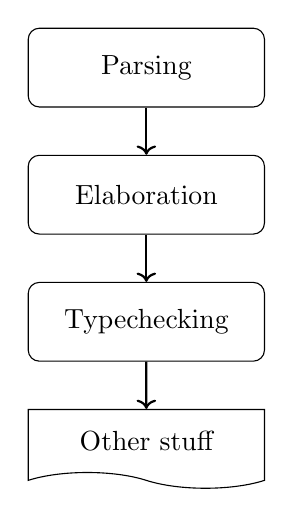
\begin{tikzpicture}[
    start chain=going below,
    every join/.style={arrow},
    node distance=0.6cm
    ]
    \node (s0) [reg, on chain, join] {Parsing};
    \node (s1) [reg, on chain, join] {Elaboration};
    \node (s2) [reg, on chain, join] {Typechecking};
    \node (s3) [end, on chain, join] {Other stuff};
  \end{tikzpicture}
  \begin{tikzpicture}[remember picture, overlay]
    \node [xshift=0.12\paperheight,yshift=0.15\paperheight] at (current page.south west){
      
\includegraphics[width=0.2\paperwidth, keepaspectratio]{mate.png}
    };
  \end{tikzpicture}
  \end{column}
  \begin{column}{0.55\textwidth}
    \pause
    \begin{itemize}[<+->]
      \item convert the user code to some very \keyword{faithful internal representation}
      \vspace{0.5em}\item translate to a \keyword{simpler}, potentially more verbose representation
      \vspace{0.2em}\item \keyword{validate} and \keyword{check} the simpler representation
      \vspace{1em}\item optimisations, environments for code execution, emitting native code, etc.
    \end{itemize}
  \end{column}
  \end{columns}
\end{frame}

%\begin{frame}{Parsing Matlab code}
%  \begin{columns}
%  \begin{column}{0.3\textwidth}
%    \begin{tikzpicture}[
%      start chain=going below,
%      every join/.style={fadearrow},
%      node distance=0.6cm
%    ]
%    \node (s0) [highlight, on chain,join] {Parsing};
%    \node (s1) [fade, on chain, join] {Elaboration};
%    \node (s2) [fade, on chain, join] {Typechecking};
%    \node (s3) [fadeend, on chain, join] {Other stuff};
%    \end{tikzpicture}
%    \begin{tikzpicture}[remember picture, overlay]
%      \node [xshift=0.12\paperheight,yshift=0.15\paperheight] at (current page.south west){
%        
\includegraphics[width=0.2\paperwidth, keepaspectratio]{mate.png}
%      };
%    \end{tikzpicture}
%  \end{column}
%  \begin{column}{0.55\textwidth}
%  Parsing actually consists of two phases --- \keyword{lexing} and \keyword{parsing}:
%  \begin{itemize}
%    \item a \keyword{lexer} converts stream of \keyword{characters} to a stream of \keyword{tokens}, e.g., by grouping digits into numbers, finding comments, etc;
%    \item a parser then converts the stream of \keyword{tokens} to an \keyword{abstract syntax tree} - a data structure amenable to further processing
%  \end{itemize}
%  There is much more to that phase...\\
%  Remark: Detecting \lr\ directive happens during lexing, i.e., very early in the pipeline.
%  \end{column}
%  \end{columns}
%\end{frame}

\begin{frame}{Core Type Theory}
  \begin{columns}
  \begin{column}{0.3\textwidth}
    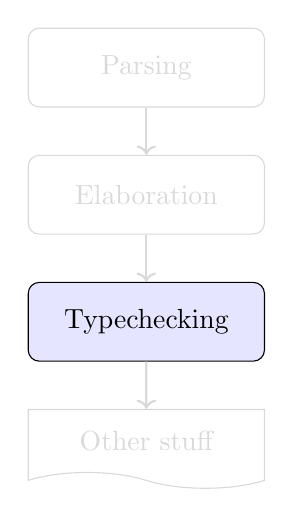
\begin{tikzpicture}[
      start chain=going below,
      every join/.style={fadearrow},
      node distance=0.6cm
      ]
      \node (s0) [fade, on chain,join] {Parsing};
      \node (s1) [fade, on chain, join] {Elaboration};
      \node (s2) [highlight, on chain, join] {Typechecking};
      \node (s3) [fadeend, on chain, join] {Other stuff};
    \end{tikzpicture}
    \begin{tikzpicture}[remember picture, overlay]
      \node [xshift=0.12\paperheight,yshift=0.15\paperheight] at (current page.south west){
        
\includegraphics[width=0.2\paperwidth, keepaspectratio]{mate.png}
      };
    \end{tikzpicture}
  \end{column}
  \begin{column}{0.55\textwidth}
    The implementation of the \keyword{algorithmic} rules of the type system. \pause
    \begin{itemize}[<+->]
      \item reports any typing \keyword{errors} during compilation
      \begin{itemize}
        \item \lr{}'s approach
      \end{itemize}
      \item but in principle can also be delayed until program execution
      \begin{itemize}
        \item to the peril of the user
        \item \ma{}'s approach
      \end{itemize}
    \end{itemize}
  \end{column}
\end{columns}
\end{frame}

\begin{frame}{A Tour of Types: Unit type}
Let's take a look at some of the types implemented in \lr{}.\pause \\
\begin{itemize}[<+->]
  \item Starting with the most important type.
  \item The type ($\Unit$) with a single inhabitant ($\star$)
  \[\star :: \Unit\]
\end{itemize}
\end{frame}

\begin{frame}{A Tour of Types: Free Abelian Groups}
\begin{itemize}[<+->]
  \item $\Abel(G)$ - the type of free Abelian groups over an arbitrary type of generators $G$
  \begin{itemize}
    \item can then define the type of integers, $\Int$, as the type $\Abel(\Unit)$.
  \end{itemize}
  \item $\Enum(xs)$ - the enumeration type for some list of constants $xs$
  \begin{itemize}
    \item letting $xs$ be the constants for length ($\LL$), time ($\TT$), and mass ($\MM$), we can model the type of \keyword{fundamental dimensions}, $\mathsf{D} := \Enum([\LL, \TT, \MM])$
  \end{itemize}
  \item An \keyword{arbitrary dimension} $d$ can be represented as an element of the free Abelian group over the type of fundamental dimensions:
  \[d :: \Abel(\mathsf{D})\]
\end{itemize}
\end{frame}


\begin{frame}[fragile]{A Tour of Types: Matrices}
\begin{itemize}[<+->]
  \item $\Matrix(T, n, m)$ - a matrix over the type of elements $T$ with dimensions $n :: \Abel(\Unit)$ and $m :: \Abel(\Unit)$
  \item good attempt, but models only \keyword{uniform matrices}
  \item many applications in metrology collect together distance, speed, acceleration, etc, in one matrix — of related, but different dimensions, e.g.,
  \[\begin{pmatrix}
    1\, \Km/\Kg & 2\, \Km/\Sec & 3\, \Km \cdot \Km \\
    4\, \Sec/\Kg & 5\, \Sec/\Sec & 6\, \Sec \cdot \Km
  \end{pmatrix}\]
\end{itemize}
\end{frame}

\begin{frame}[fragile]{A Tour of Types: Matrices}
\begin{itemize}[<+->]
  \item $\Matrix(R, C, T, rs, cs)$
  \begin{itemize}
  \item $rs$ and $cs$ - row and column headers
  \item $R$, $C$ - types of the elements in the row and column headers
  \item $T$ - type of the cell entries in the matrix
  \end{itemize}
  \item very similar representation to a spreadsheet
  \begin{center}
    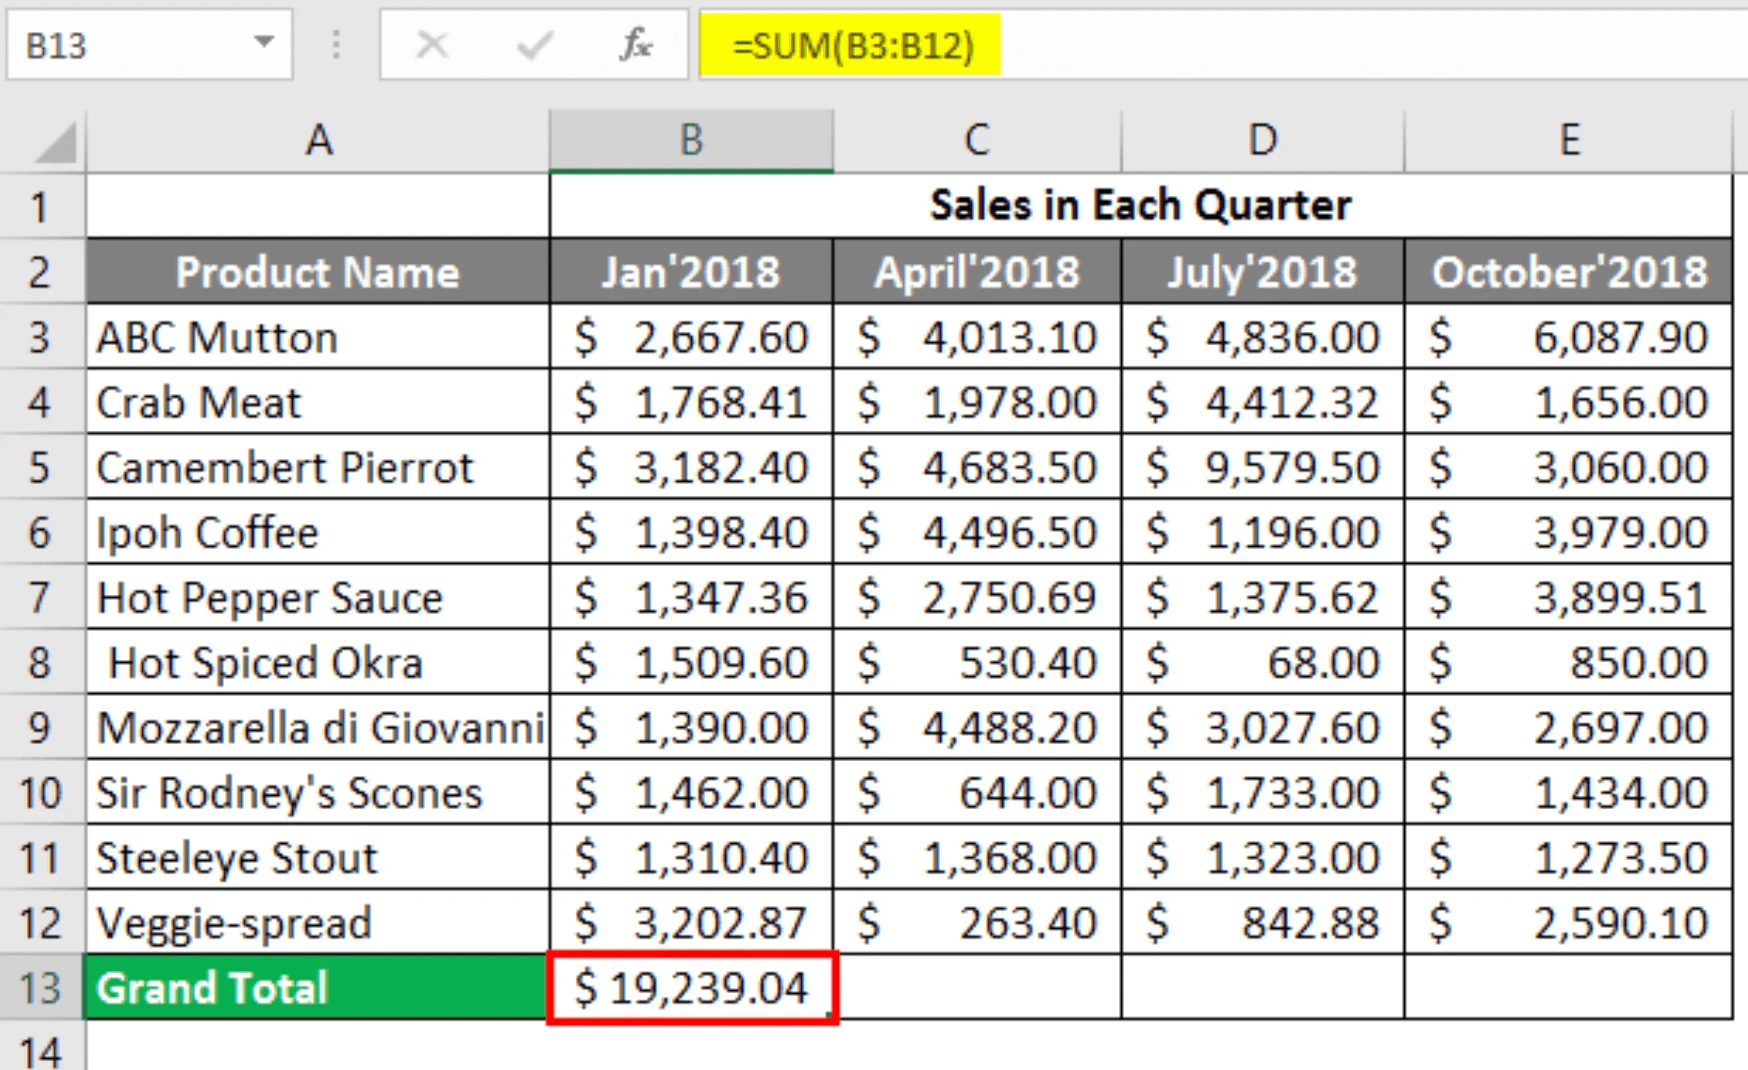
\includegraphics[width=0.7\linewidth]{spreadsheet}
  \end{center}

\end{itemize}
\end{frame}

\begin{frame}{Elaborating Matlab expressions to CoreTT}
  \begin{columns}
  \begin{column}{0.3\textwidth}
    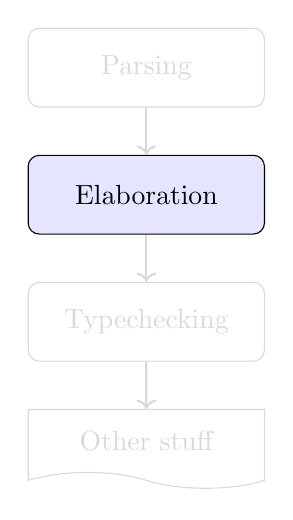
\begin{tikzpicture}[
      start chain=going below,
      every join/.style={fadearrow},
      node distance=0.6cm
      ]
      \node (s0) [fade, on chain,join] {Parsing};
      \node (s1) [highlight, on chain, join] {Elaboration};
      \node (s2) [fade, on chain, join] {Typechecking};
      \node (s3) [fadeend, on chain, join] {Other stuff};
    \end{tikzpicture}
    \begin{tikzpicture}[remember picture, overlay]
      \node [xshift=0.12\paperheight,yshift=0.15\paperheight] at (current page.south west){
        
\includegraphics[width=0.2\paperwidth, keepaspectratio]{mate.png}
      };
    \end{tikzpicture}
  \end{column}
  \begin{column}{0.55\textwidth}
    The \keyword{interface} between the type system and the user written code. \pause
    \begin{itemize}[<+->]
      \item tries to fill the gaps between the two
      \begin{itemize}
        \item e.g., comes up with types for \ma{} expressions
      \end{itemize}
      \item makes sure that type errors are human readable
    \end{itemize}
  \end{column}
\end{columns}
\end{frame}


\begin{frame}[fragile]{Elaborating Assignments}
  \begin{lstlisting}[xleftmargin=10em]
    %> n!\tikzmark{ndecl}! :: int!\tikzmark{intdecl}!
    n !\tikzmark{nlhs}!=!\tikzmark{ass1}! 5!\tikzmark{five}!;
    x !\tikzmark{xlhs}!=!\tikzmark{ass2}! n !\tikzmark{nrhs}!
    %> typeof x!\tikzmark{xtypeof}!
  \end{lstlisting}
  \pause
  \mycallout<+>{ndecl}{see a new variable $n$}
  \mycallout<+>{intdecl}{simplify $n$'s type}
  \mycallout<+>{ndecl}{declare $n$ in scope with type $int$}
  \mycallout<+>{ass1}{see an assignment at yet unknown type}
  \mycallout<+>{five}{process the RHS, $5$, using the the type of LHS $n$}
  \mycallout<+>{nlhs}{find the type of the declared $n$}
  \mycallout<+>{ass1}{constrain the type of RHS, $5$, to be equal to that of LHS, $n$}
  \mycallout<+>{ass2}{see an assignment at yet unknown type}
  \mycallout<+>{nrhs}{simplify the RHS, $n$, finding its type}
  \mycallout<+>{xlhs}{declare $x$ in scope with unknown type}
  \mycallout<+>{ass2}{constrain the type of RHS, $n$, to be equal to that of LHS, $x$}
  \mycallout<+>{xtypeof}{find the type of the declared $x$}
\end{frame}

\begin{frame}[fragile]{Current Progress}
  \begin{itemize}[<+->]
    \item The code is available at \repo
    \item We are currently parsing a lot of common \ma{} constructions
    \item Directives for renaming and code generation are working
    \item Implemented most of the underlying type system for \ma
    \item Actively working on elaboration
  \end{itemize}
  \pause
  \vspace{3em}
  \LARGE \centerline{Thank you for your attention!}
\end{frame}

%\begin{frame}[allowframebreaks]
%  \frametitle{References}
%  \printbibliography
%\end{frame}

\end{document}
%%% Local Variables:
%%% mode: latex
%%% TeX-master: t
%%% End:
